\chapter{Understanding phytoplankton community shifts in the eastern Cariaco basin}

\small {\textbf{This is the current state of progress towards the first manuscript}}


\normalsize
\section{Regime shift in the Cariaco Basin}
The CARIACO time-series has been collecting detailed data on the phytoplankton community in the Cariaco Basin from 1995 to 2017 (see Section \ref{CARIACOintro} for a full description). What has been a particular focus of the research based on this data set is the apparent changes in environmental conditions documented in both the physical boundary conditions as well as the biological data. 
As documented by \citet{Taylor2012}

and further investigated by \citet{Pinckney2015}

Interesting thing is that there was this shift in the PhytoplanktonCommunity but apparently no real reduction in Export! (This is in Taylor and Pinckney somehwere)
this would be coherent with Pinckney, no real reduction in biomass, but shifts in the community and towards greater depth, talk about depth of the euphotic zone! also have that data thanks to JP and CBN

\begin{figure}
\centering
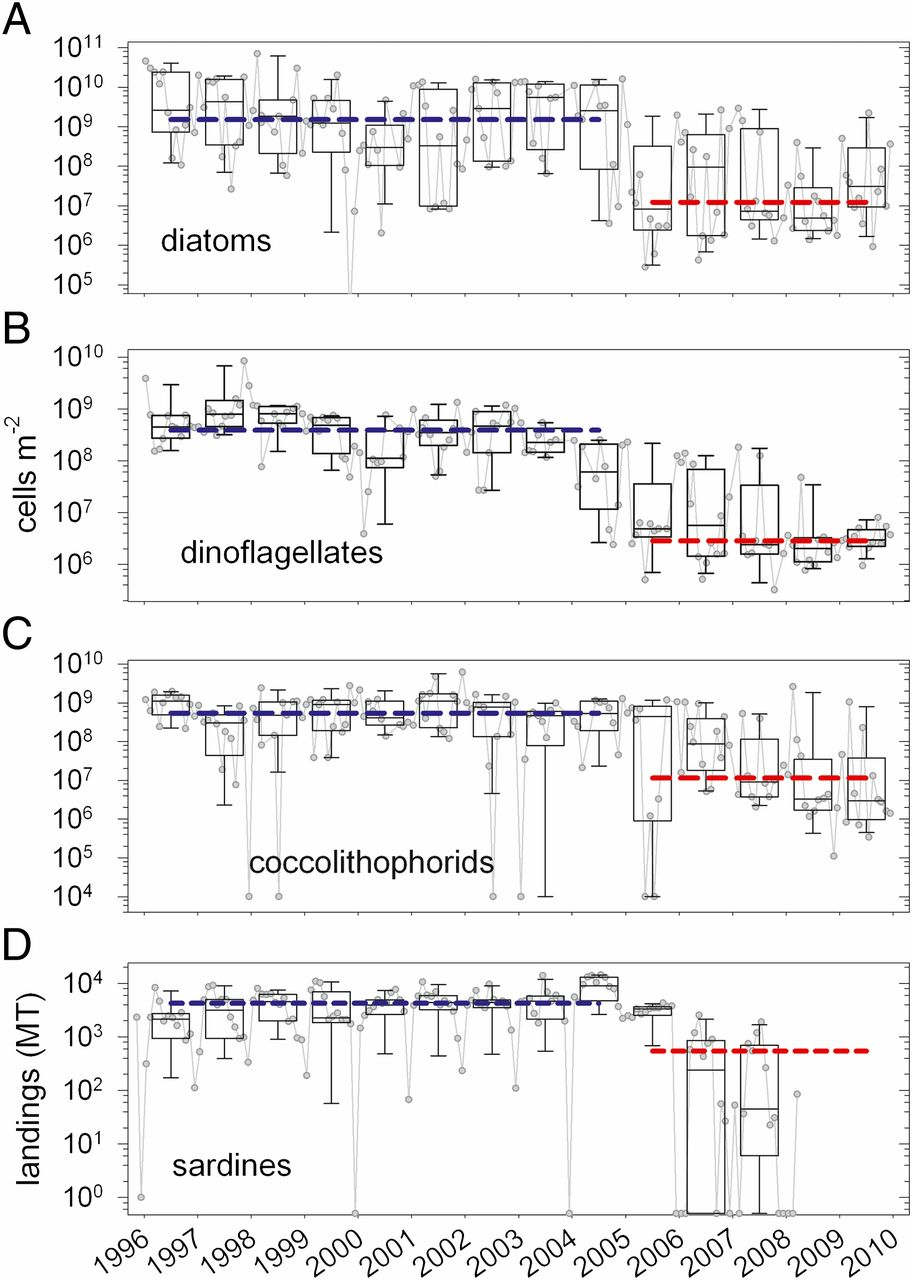
\includegraphics[trim = 0mm 0mm 0mm 0mm, clip, width=0.7\linewidth]{./Chp2-Pre/Tayloretal2012_F3.large.jpg}
\caption[Scheme]{\small {"Shifts in phytoplankton community composition and sardine landings from the southeastern Margarita Island fishery. Monthly observations presented as gray symbols. Box and whisker plots depict binned annual variations in diatom (A), dinoflagellate (B), coccolithophorid (C) inventories integrated over the upper 55 m and sardine fishery landings (D) in metric tons. Boxes represent the interquartile range of all observations (25th to 75th percentiles). Internal horizontal lines and whiskers are medians and 10th to 90th percentiles, respectively. Blue and red horizontal lines represent the grand medians of all observations between 1996 and 2004 and between 2005 and 2009, respectively. Data in early and late bins are significantly different in all cases (ANOVA; P < 0.001). [Fishery data are courtesy of L. W. Gonzáles (Universidad de Oriente, Boca de Río, Isla de Margarita, Venezuela); zero values artificially set at 0.5 for plotting purposes.)" from \citet{Taylor2012}}}
\label{PrinComp}
\end{figure}




The term regime shift is actually not very well defined and has been used... \citep{DeYoung2004a}
There are global trends and indications of a regime shift, but methods to identify regime shifts are not well established and have been critically discussed in the literature \citep{Steele2004a, Mantua2004a, Litzow2016a}. To my knowledge no formal exploration of a potential regime shift has been performed with the CARIACO data, therefore the term regime shift is used here to describe the observed changes in the phytoplankton community and physical environment without presupposing a formally defined state shift in the entire ecosystem. 


\begin{figure}
\centering
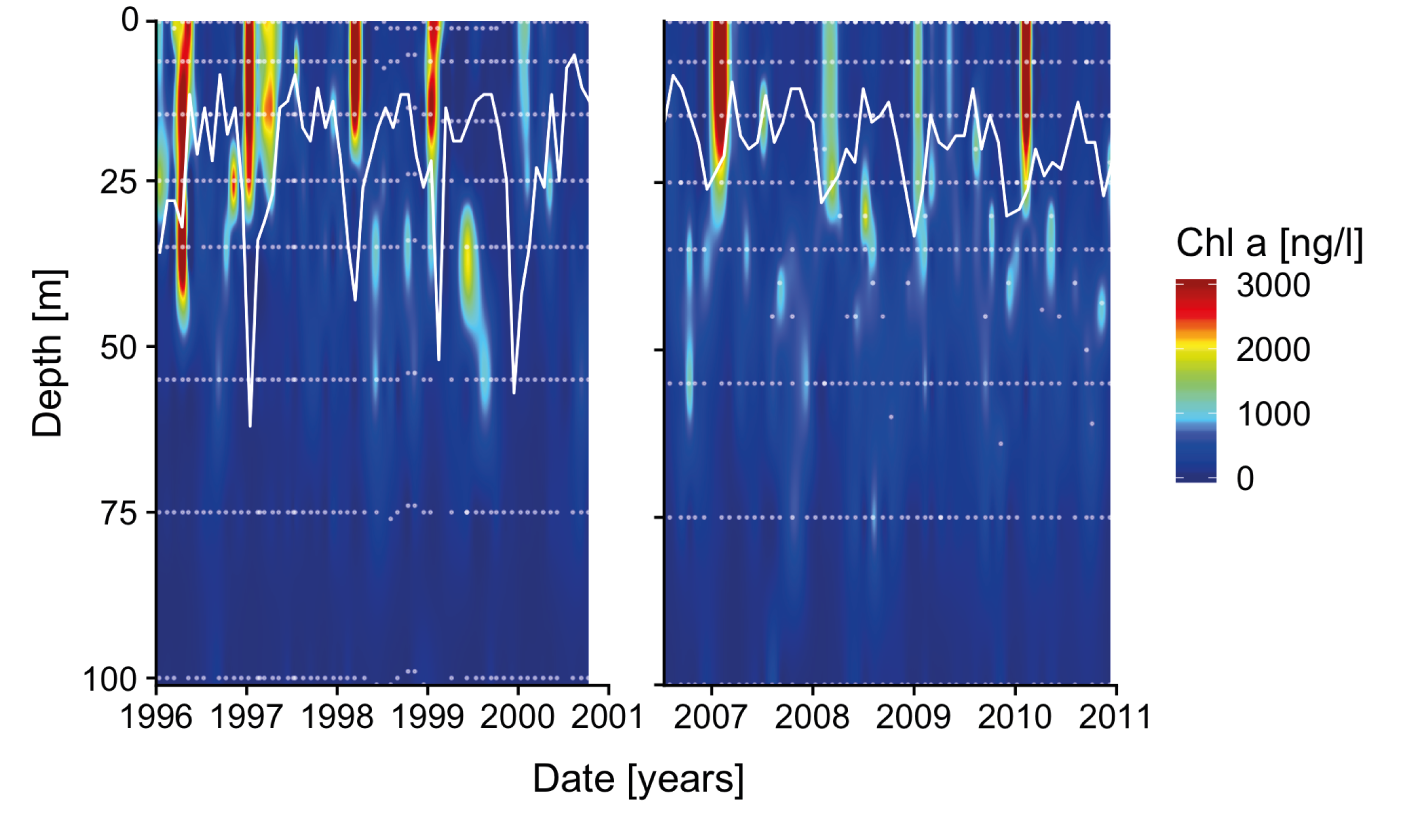
\includegraphics[trim = 0mm 0mm 0mm 0mm, clip, width=.9\linewidth]{./Chp2-Pre/Pinckneyetal2015_TotChlAcontoursMLD.png}
\caption[Scheme]{\small {Contour plot of HPLC-measured $chl~a$ for the two time periods with full data coverage (January 1996 to October 2000 and July 2006 to December 2010). Light white dots indicate data points. White line shows the depth of the mixed layer. HPLC Data and MLD depth was received from James Pinckney and Claudia Benitez-Nelson.}}
\label{PrinComp}
\end{figure}


Talk about the data again

Also talk about mutshinda et al studies!
Mutshinda study one, bayesian approach: \cite{Mutshinda2013a}

Mutshinda study, same year, environmental factors: \cite{Mutshinda2013}

culminated in the study in PNAS: "Phytoplankton adapt to a changing environment" \cite{Irwin2015}

detailed phytoplankton data has been used in the previous studies for statistical analysis, but suprisingly not yet for ecosystem or trait-based modeling
This will be a first! first proper ecological model apart from this Export Flux model only including diatoms \citep{Walsh2002a}

FUNCTIONAL TYPES STRUCTURE --> explain linkage between Pigment Data that I use and functional diversity measurements (XMoreno et al. 2012X) take this from Pinckney et al. 2015...
Thus, photopigment-based measures offer an efficient way to quantify community or functional diversity (X Moreno et al., 2012 X). (From Pinckney et al 2015) ..> this would also be good to discuss in part 4!

bb


LOOKING AT BIOMASS DYNAMICS, leading over from Intro where i mentioned JP CBN data at the end (ad-lib)
XXX

EXPLAIN THE HYPOTHESES HERE; AND HOW THEY CAN BE TESteD

Main hypothesis, based on top down and bottom up processes:
Top down grazing has great influence on ecosystem, not just from biomass, but also biodiversity aspects \cite{Prowe2012c}.


\section{Methods}

MODEL STRUCTURE: 

- Cyanos as of yet not implemented as nitrogen fixers, given simplicity of model formulation, but actually are present and could be included: \citep{Montes2013}

dont really go into depth here, just generally state how things are done, python, odeint, system of ODEs

COPY METHODS SECTION FROM PhytoSFDM in a way, but with the current model setup
including the equations and allofthat!

SHOW MODEL SCHEMATICS!

XXXX

\small {\textbf{Model physics in a tropical coastal setting}}

xXXX

Most models built for temperate oceans, since that is where reasearch (and funding) has been most well developed. Fasham NPZD type slabe physics explain.
Why won't this fit well in the Cariaco setting? - mostly due to shallow and comparatively invariable MLD, and nutrient fluxes don't correlate.
Problem of nutrient forcing! If MLD driven, nutrients below MLD are highly variable, only below 100m do we get towards a relatively constant N0 and Si0 (can show plots here!)

Moved from slab physics of PhytoSFDM model \citep{Acevedo-Trejos2016} which is based on Fasham \citep{Evans2003,Fasham1990a} to a box model formulation adapted from Tyrrell \citep{Tyrrell1999}
The specific differences are (show equations):

HERE I CAN SHOW THE DIFFERENT MODEL RUNS, explain the difference
for this box model needs to get running! This won't be so easy.. so plan ample time my friend!

XXXX

XXXX

XXX


End Methods here

\section{Preliminary Results}


SHOW PROPER RUN, With Biotic components fitting the base run comparatively well, try it!

XXXX (Figure \ref{RegSizeFrac}).



$kkkkkkkkkkkkkkkkkkkkkk$ here the results start, at least the text of it

$^{\circ}$C$^{\circ}$\%$^{\circ}$C$^{\circ}$\%$^{\circ}$C$^{\circ}$\%$^{\circ}$C$^{\circ}$\%


get it, get it



